\section{Paketverlust erkennen}
\label{sec:Paketverlust erkennen}

\subsection{Einleitung}

{\raggedright
Falls ein \"{U}bertragungsmedium nicht korrekt funktioniert ist es m\"{o}glich,
dass Datenpakete nicht am Ziel ankommen oder mit einer zu grossen Versp\"{a}tung.
Da jedes \esp Paket mit einer Sequenznummer versehen ist, k\"{o}nnen diese
Paketverluste erkannt und gemeldet werden.
}

{\raggedright
Die \esp Pakete Besitzen zum Schutz vor Replay-Angriffen eine Sequenznummer sowie
einen bestimmten G\"{u}ltigkeitsbereich (Windowsize).
\\
Die Pakete k\"{o}nnen zum Beispiel durch Loadbalancing \"{u}ber unterschiedliche
Pfade verschickt werden. Dadurch kann die Reihenfolge der Pakete am Ziel nicht
mehr gew\"{a}hrleistet werden. Die zu sp\"{a}t ankommenden Pakete m\"{u}ssen
daher \"{u}berpr\"{u}ft werden, ob die Sequenznummer aktuell noch g\"{u}ltig ist
(innerhalb des Window).
}

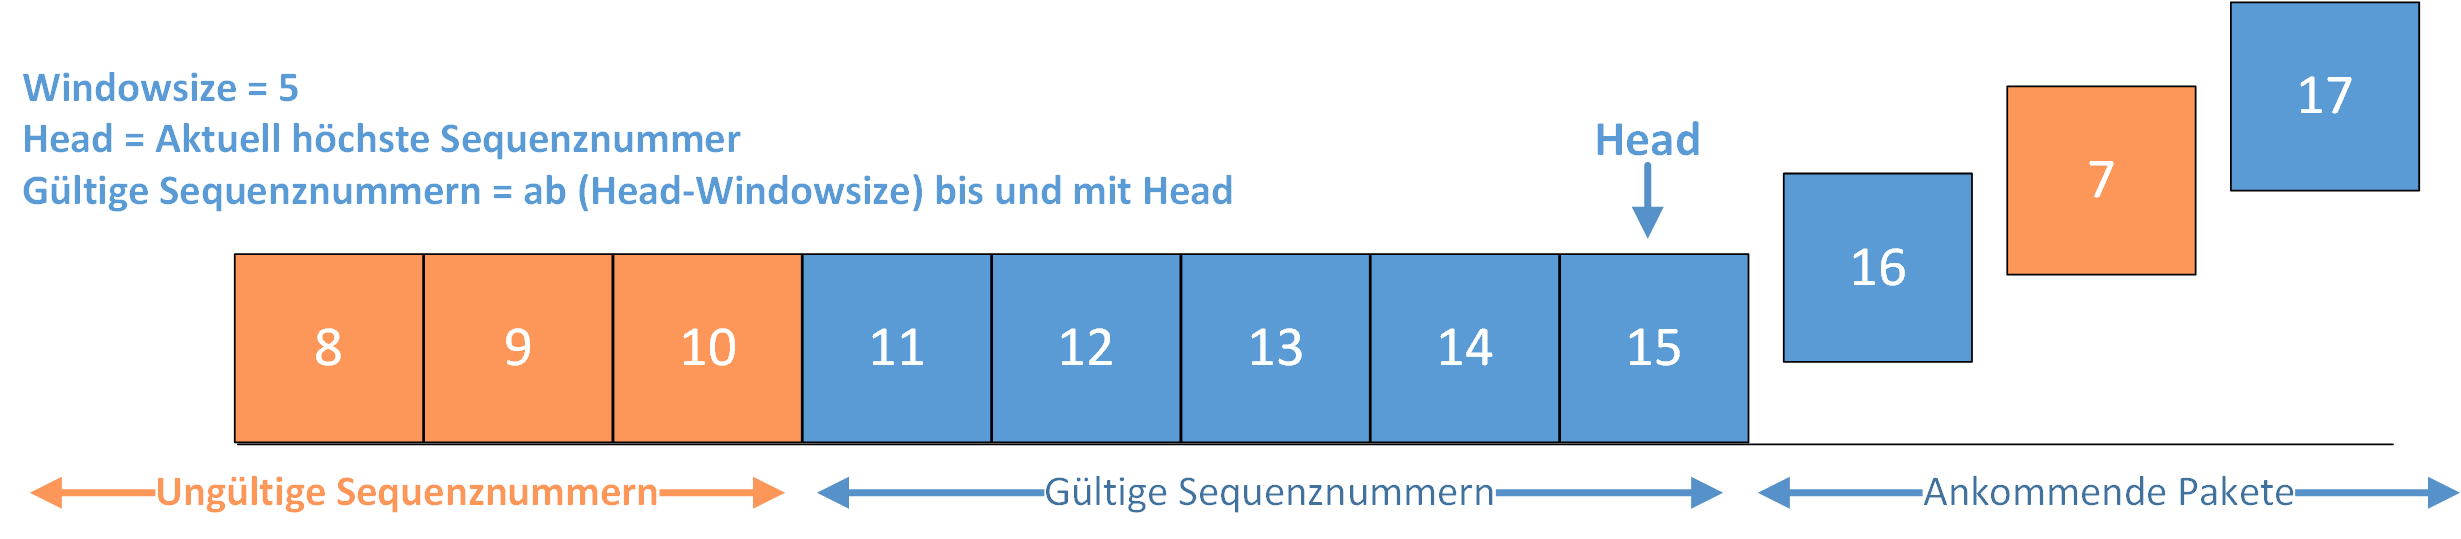
\includegraphics[width=1\textwidth]{start/img/Sequenznummern.png}

\subsection{Datenstruktur für die \esp Verbindungen}
Da pro Verbindung separate Sequenznummern verwendet werden, werden die verschiedenen Verbindungen durch eine Hashmap verwaltet. Als Key wird eine Struktur aus Source, Destination und \acs{SPI} verwendet. Als Value werden grundsätzlich zwei Listen für die Lost und MaybeLost Pakete benötigt. Zusätzlich wird noch ein Wert für den aktuellen Head gespeichert.

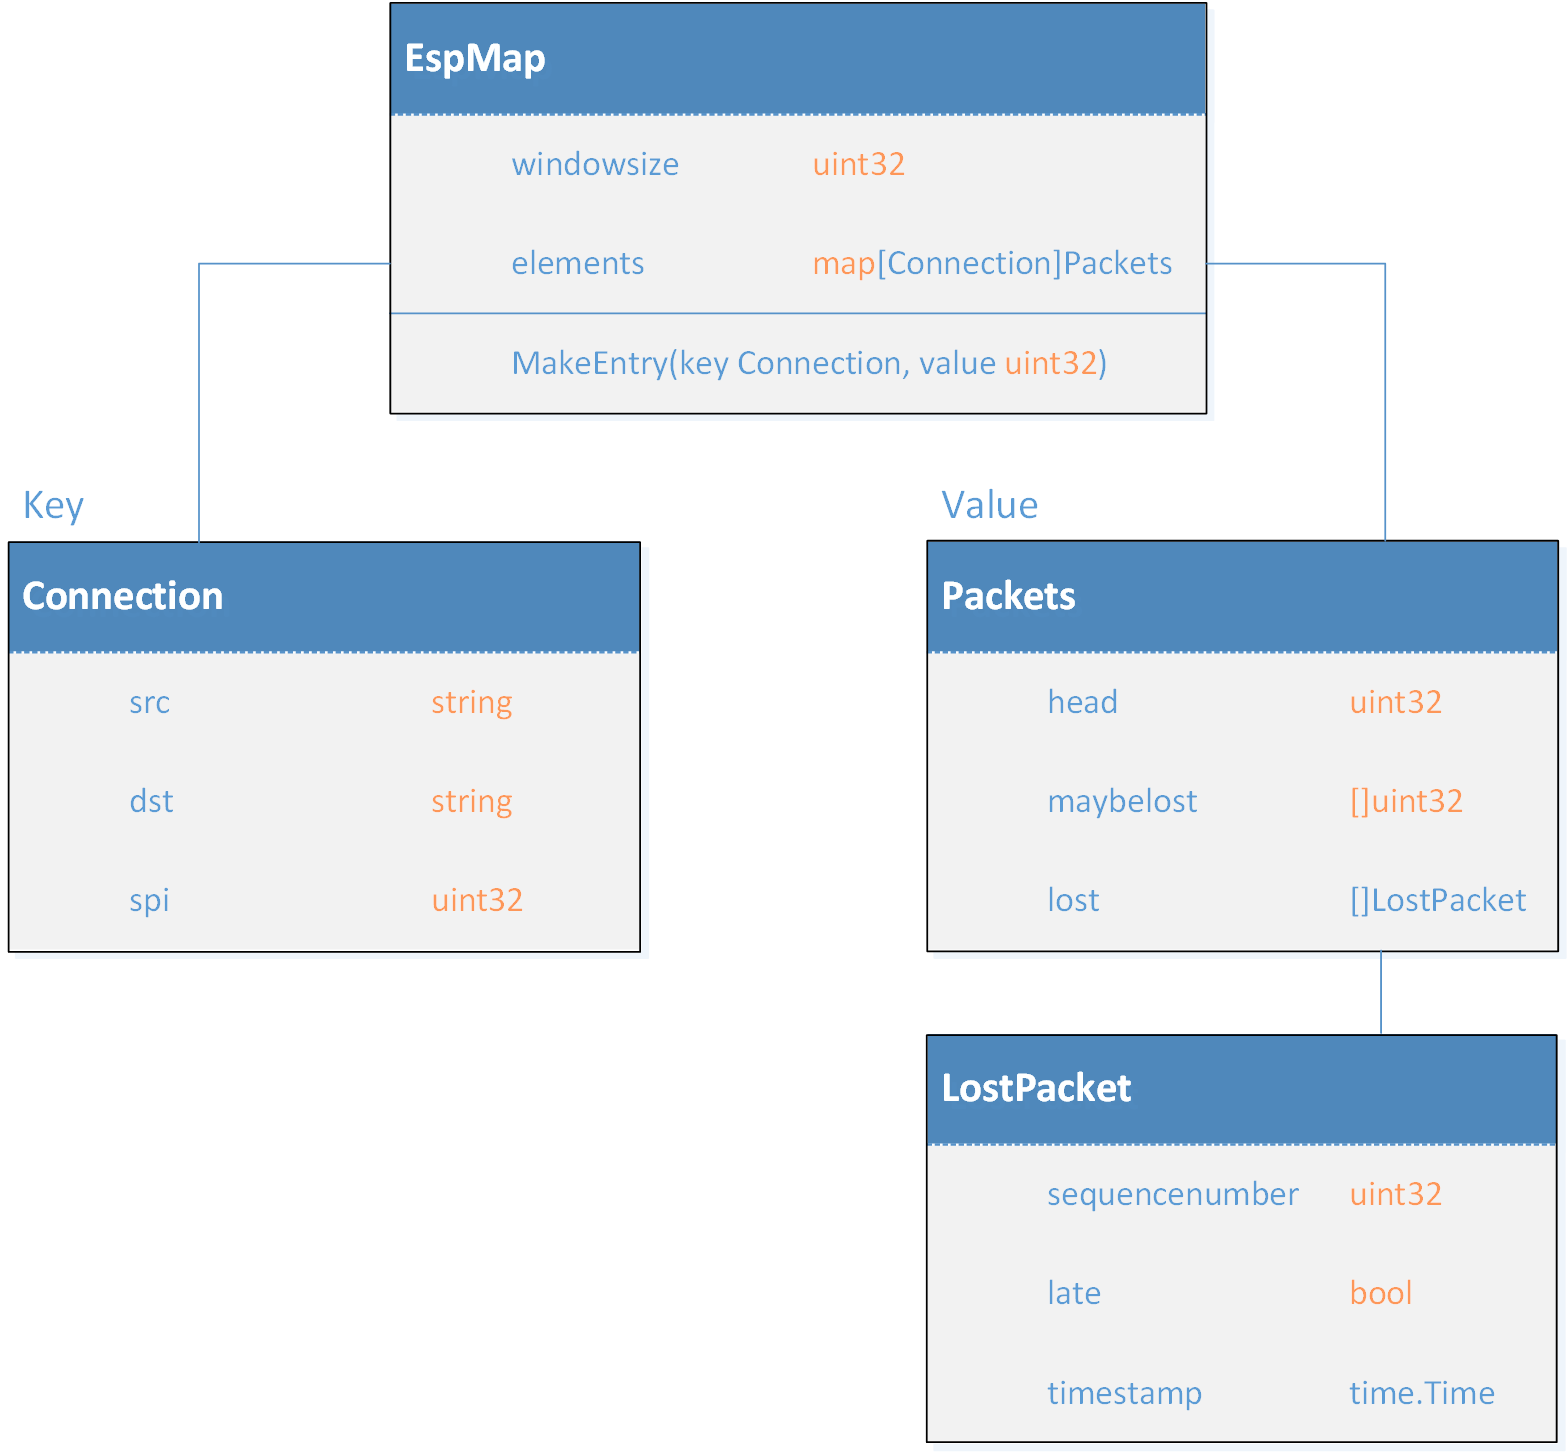
\includegraphics[width=1\textwidth]{start/img/Datenstruktur.png}

\subsection{Erkennung des Paketverlusts}
Die Paketverluste werden mit folgendem Algorithmus festgestellt.
Vereinfachte Darstellung des Algorithmus in Pseudocode:
\\
\textbf{Neues Packet Verarbeiten}
\begin{lstlisting}[language=go]
if(neuesPacket > Head){
	if(neuesPacket != Head + 1){
		Packete von Head bis neuesPacket in 
		MaybeLost speichern
	}
	Head = neuesPacket
	CheckLost()
}else{
	if(Head-WindowSize < neuesPacket){
		Packet aus MaybeLost entfernen
	}else{
		Flag fuer zu spaet angekommen setzen	
	}
}
\end{lstlisting}

\textbf{CheckLost}
\begin{lstlisting}[language=go]
for(MaybeLost){
	if(Head-WindowSize >= MaybeLostEintrag){
		Packet in Lost Speichern
		Packet aus MaybeLost entfernen
	}
}
\end{lstlisting}
